\chapter{Model Physics}
\label{chap:landice-physics}


% ===============================
% ===================================================
%\section{Model Physics}
% ===============================
% ===============================

Physical processes currently implemented in MALI are a mass-conserving subglacial hydrology model and a small number of basic schemes for iceberg calving. These are described in more detail below.

% ===============================
\section{Subglacial Hydrology}
% ===============================
\label{sec:subglacialHydro}

Sliding of glaciers and ice sheets over their bed can increase ice velocity by orders of magnitude
and is the primary control on ice flux to the oceans.
The state of the subglacial hydrologic system is the primary control on sliding \citep{Clarke2005, Cuffey2010, Flowers2015},
and ice sheet modelers have therefore emphasized subglacial hydrology and its effects on basal sliding 
as a critical missing piece of current ice sheet models \citep{Little2007, Price2011a}.
%Despite the fact that the sliding of ice sheets over their bed is the primary control on ice flux to the oceans, current ice sheet models reduce this process to a single parameter that cannot evolve4?7.

MALI includes a mass-conserving model of subglacial hydrology that includes representations of any or all of
water storage in till, distributed drainage, and channelized drainage and is coupled to ice dynamics.
The model is based on the model of \citet{Bueler2015} with an additional component for channelized drainage
and modified for MALI's unstructured horizontal grid.  
While the implementation follows closely that of \citet{Bueler2015}, the model and equations are summarized here
along with a description of the features unique to the application in MALI.

% --- overview of each system ----

% till
\subsection{Till}
The simple till component represents local storage of water in subglacial till without horizontal transport within the till.  
Evolution of the effective water depth in till, $W_{till}$ is therefore a balance of delivery of meltwater, $m_b$, to the till, drainage of water out of the till at rate $C_d$ (mass leaving the subglacial hydrologic system, for example, to deep groundwater storage), and overflow to the distributed drainage system, $\gamma$:
\begin{equation}
   \frac{\partial W_{till}}{\partial t} = \frac{m_b}{\rho_w} - C_d - \gamma_t.
\label{sgh:tillevol}
\end{equation}
In the model, meltwater (from either the bed or drained from the surface), is first delivered to the till component.  
Water in excess of the the maximum storage capacity of the till, $W_{till}^{max}$,
is instantaneously transferred as a source term to the distributed drainage system through the $\gamma_t$ term.

% distributed drainage
\subsubsection{Distributed drainage}
The distributed drainage component is implemented as a ``macroporous sheet'' that represents 
bulk flow through linked cavities that form in the lee of bedrock bumps as the glacier slides over the bed \citep{Flowers2002a, Hewitt2011, Flowers2015}.
Water flow in the system is driven by the gradient of the hydropotential, $\phi$, defined as
\begin{equation}
   \phi = \rho_w g z_b + P_w
\label{sgh:phi}
\end{equation}
where $P_w$ is the water pressure in the distributed drainage system.
A related variable, the ice effective pressure, $N$, is the difference between ice overburden pressure and water pressure in the distributed drainage system, $P_w$:
\begin{equation}
   N = \rho g H - P_w .
\label{sgh:N}
\end{equation}

The evolution of the area-averaged cavity space is a balance of 
opening of cavity space by the glacier sliding over bedrock bumps 
and closing through creep of the ice above.
The model uses the commonly used assumption \citep[e.g.][]{Schoof2010a,Hewitt2011,Werder2013,Hoffman2014} 
that cavities always remain water filled \citep[c.f.][]{Schoof2012},
so cavity space can be represented by the effective water depth in the macorporous sheet, $W$:
\begin{equation}
   \frac{\partial W}{\partial t} = c_s |\vec{u_b}| (W_r - W) - c_{cd} A_b N^3 W
\label{sgh:cavityevol}
\end{equation}
where $c_s$ is bed roughness parameter, $W_r$ is the maximum bed bump height,
$c_{cd}$ is creep scaling parameter representing geometric and possibly other effects, 
and $A_b$ is the ice flow parameter of the basal ice.

Water flow in the distributed drainage system, $\vec{q}$, is driven the hydropotential gradient and is described by a general power-law:
\begin{equation}
   \vec{q} = -k_q W^{\alpha_1} |\nabla \phi|^{\alpha_2-2} \nabla \phi 
\label{sgh:q}
\end{equation}
where $k_q$ is a conductivity coefficient. 
The $\alpha_1$ and $\alpha_2$ exponents can be adjusted so that Eq. \ref{sgh:q} reduces to 
commonly used water flow relations, such as Darcy flow, the Darcy-Weisbach relation, and the Manning equation.

% channelized drainage
\subsection{Channelized drainage}
The inclusion of channelized drainage in MALI is an extension to the model of \citet{Bueler2015}.
The distributed drainage model ignores dissipative heating within the water,
which in the real world leads to melting of the ice roof, and the formation of discrete, efficient
channels melted into the ice above when the distributed discharge reaches a critical threshold \citep{Schoof2010a, Hewitt2011, Werder2013, Flowers2015}.
These channels can rapidly evacuate water from the distributed drainage system and 
lower water pressure, even under sustained meltwater input \citep{Schoof2010a, Hewitt2011, Werder2013, Hoffman2014, Flowers2015}.

The implementation of channels follows the channel network models of \citet{Werder2013} and \citet{Hewitt2013}.
The evolution of channel area, $S$, is a balance of opening and closing processes 
as in the distributed system, but in channels the opening mechanism is 
melting caused by dissipative heating of the ice above:
\begin{equation}
   \frac{dS}{dt} = \frac{1}{\rho L} ( \Xi - \Pi ) - c_{cc} A_b N^3 S
\label{sgh:channelevol}
\end{equation}
where $c_{cc}$ is the creep scaling parameter for channels.

The channel opening rate, the first term in Eq. \ref{sgh:channelevol}, 
is itself a balance of dissipation of potential energy, $\Xi$, 
and sensible heat change of water, $\Pi$, due to changes in the pressure-dependent melt temperature.
Dissipation of potential energy includes energy produced by flow in both the channel itself 
and a small region of the distributed system along the channel:
\begin{equation}
   \Xi = \left| \frac{d\phi}{ds}\vec{Q} \right|  +  \left| \frac{d\phi}{ds}\vec{q_c} l_c \right| 
\label{sgh:channeldissip}
\end{equation}
where $s$ is the spatial coordinate along a channel segment, 
$\vec{Q}$ is the flow rate in the channel, and
$\vec{q_c}$ is the flow in the distributed drainage system parallel to the channel
within a distance $l_c$ of the channel.
The term adding the contribution of dissipative melting within the distributed drainage system
near the channel is included to represent some of the energy that has been ignored from that process 
in the description of the distributed drainage system 
and allows channels to form even when channel area is initially zero 
if discharge in the distributed drainage system is sufficient \citep{Werder2013}.
The term representing sensible heat change of the water, $\Pi$, is necessitated by the 
assumption that the water always remains at the pressure-dependent melt temperature
of the water.
Changes in water pressure must therefore result in melting or freezing:
\begin{equation}
   \Pi = -c_t c_w \rho_w \left(\vec{Q} + l_c \vec{q_c} \right) \frac{d P_w}{d s} 
\label{sgh:channelfreeze}
\end{equation}
where $c_t$ is the Clapeyron slope and $c_w$ is the specific heat capacity of water.
%{\color{red}\textbf{(TODO remove if defined above)}}.
The pressure-dependent melt term can be disabled in the model.

Water flow in channels, $\vec{Q}$, mirrors Eq. \ref{sgh:q}:
\begin{equation}
   \vec{Q} = -k_Q S^{\alpha_1} |\nabla \phi|^{\alpha_2-2} \nabla \phi 
\label{sgh:Q}
\end{equation}
where $k_Q$ is a conductivity coefficient for channels. 


% combined eqns
\subsection{Drainage component coupling}
Eqs. \ref{sgh:tillevol}-\ref{sgh:Q} are coupled together by describing the drainage system with two equations,
mass conservation and pressure evolution.
Mass conservation of the subglacial drainage system is described by
\begin{equation}
 \frac{\partial W}{\partial t} +  \frac{\partial W_{till}}{\partial t} = 
    - \nabla \cdot (\vec{V_d} W) + \nabla \cdot (D_d \nabla W) 
    - \left[ \frac{\partial S}{\partial t} + \frac{\partial Q}{\partial s} \right] \delta(x_c)
    + \frac{m_b}{\rho_w}
\label{sgh:masscon}
\end{equation}
where 
$V_d$ is water velocity in the distributed flow, $D_d$ is the diffusivity of the distributed flow, 
and $\delta(x_c)$ is the Dirac delta function applied along the locations of the linear channels.

Combining Eq. \ref{sgh:masscon} and Eq. \ref{sgh:cavityevol} and making the simplification that cavities remain full at all times 
yields an equation for water pressure within the distributed drainage system, $P_w$:
\begin{equation}
 \frac{\phi_0}{\rho_w g} \frac{\partial P_w}{\partial t} =
    - \nabla \cdot \vec{q} 
    +  c_s |\vec{u_b}| (W_r - W) - c_{cd} A_b N^3 W
    - \left[ \frac{\partial S}{\partial t} + \frac{\partial Q}{\partial s} \right] \delta(x_c)
    + \frac{m_b}{\rho_w}
    - \frac{\partial W_{till}}{\partial t}
\label{sgh:pressure}
\end{equation}
where $\phi_0$ is an englacial porosity used to regularize the pressure equation.
Following \citet{Bueler2015}, the porosity is only included in the pressure equation
and is excluded from the mass conservation equation.

Any of the three drainage components (till, distributed drainage, channelized drainage) can be deactivated at runtime.  
The most common configuration currently used is to run with distributed drainage only.

% implementation to FVM, b.c., etc.
\subsection{Numerical implementation}

The drainage system model is implemented using Finite Volume Methods on the unstructured grid used by MALI.  
State variables ($W, W_{till}, S, P_w$) are located at cell centers and 
velocities and fluxes ($\vec{q}, \vec{V_d}, \vec{Q}$) are calculated at edge midpoints.
Channel segments exist along the lines joining neighboring cell centers.
Eq. \ref{sgh:masscon} is evaluated by summing tendencies from discrete fluxes into or out of each cell.
First-order upwinding is used for advection.
At land-terminating ice sheet boundaries, $P_w=0$ is applied as the boundary condition.
At marine-terminating ice sheet boundaries, the boundary condition is $P_w=-\rho_w g z_b$, where $\rho_w$ is ocean water density.
The drainage model uses explicit forward Euler time-stepping using 
Eqs. \ref{sgh:tillevol}, \ref{sgh:masscon}, \ref{sgh:channelevol}, and \ref{sgh:pressure}.
This requires obeying advective and diffusive Courant-Friedrichs-Lewy (CFL) conditions for distributed drainage as described by \cite{Bueler2015}, 
as well as an additional advective CFL condition for channelized drainage, if it is active.

We acknowledge that the non-continuum implementation of channels can make the solution
grid-dependent, and grid convergence may therefore not exist for many problems \citep{Bueler2015}.
However, for realistic problems with irregular bed topography, we have found dominant
channel location is controlled by topography, mitigating this issue.

% coupling to MALI
\subsection{Coupling to ice sheet model}
\label{sec:sgh-coupling}

The subglacial drainage model is coupled to the ice dynamics model through a basal friction law.
Currently, the only option is a modified Weertman-style power law \citep{Bindschadler1983,Hewitt2013} that adds a term for effective pressure to Eq. \ref{eq:basalBC}:
\begin{equation}
 \vec{\tau_b} = C_0 N \vec{u_b}^m
\label{sgh:frictionlaw}
\end{equation}
where $C_0$ is a friction parameter.
Implementation of a Coulomb friction law \citep{Schoof2005, Gagliardini2007}
and a plastic till law \citep{Tulaczyk2000a,Bueler2015} are in development.
When the drainage and ice dynamics components are run together,
coupling of the systems allows the negative feedback described by \citep{Hoffman2014}
where elevated water pressure increases ice sliding and increased sliding opens additional cavity space, lowering water pressure.
The meltwater source term, $m$, is calculated by the thermal solver in MALI.
Either or both of the ice dynamics and thermal solvers can be disabled, 
in which case the relevant coupling fields can be prescribed to the drainage model.

% verification/validation
\subsection{Verification and Real-world Application}

To verify the implementation of the distributed drainage model, we use the nearly exact solution described by \citet{Bueler2015}.
The problem configuration uses distributed drainage only on a two-dimensional, radially-symmetric ice sheet of radius 22.5 km with parabolic ice sheet thickness and a nontrivial sliding profile.  
\citet{Bueler2015} showed that this configuration allows for nearly-exact reference values of $W$ and $P_w$
to be solved at steady state from an ordinary differential equation initial value problem with very high accuracy.
We follow the test protocol of \citet{Bueler2015} and initialize the model
with the near-exact solution and then run the model forward for one month,
after which we evaluate model error due to drift away from the expected solution.
Performing this test with the MALI drainage model, 
we find error comparable to that found by \citet{Bueler2015} and 
approximately first order convergence (Figure \ref{fig:sgh:radialsolnfig}).

\begin{figure}[t]
\centering
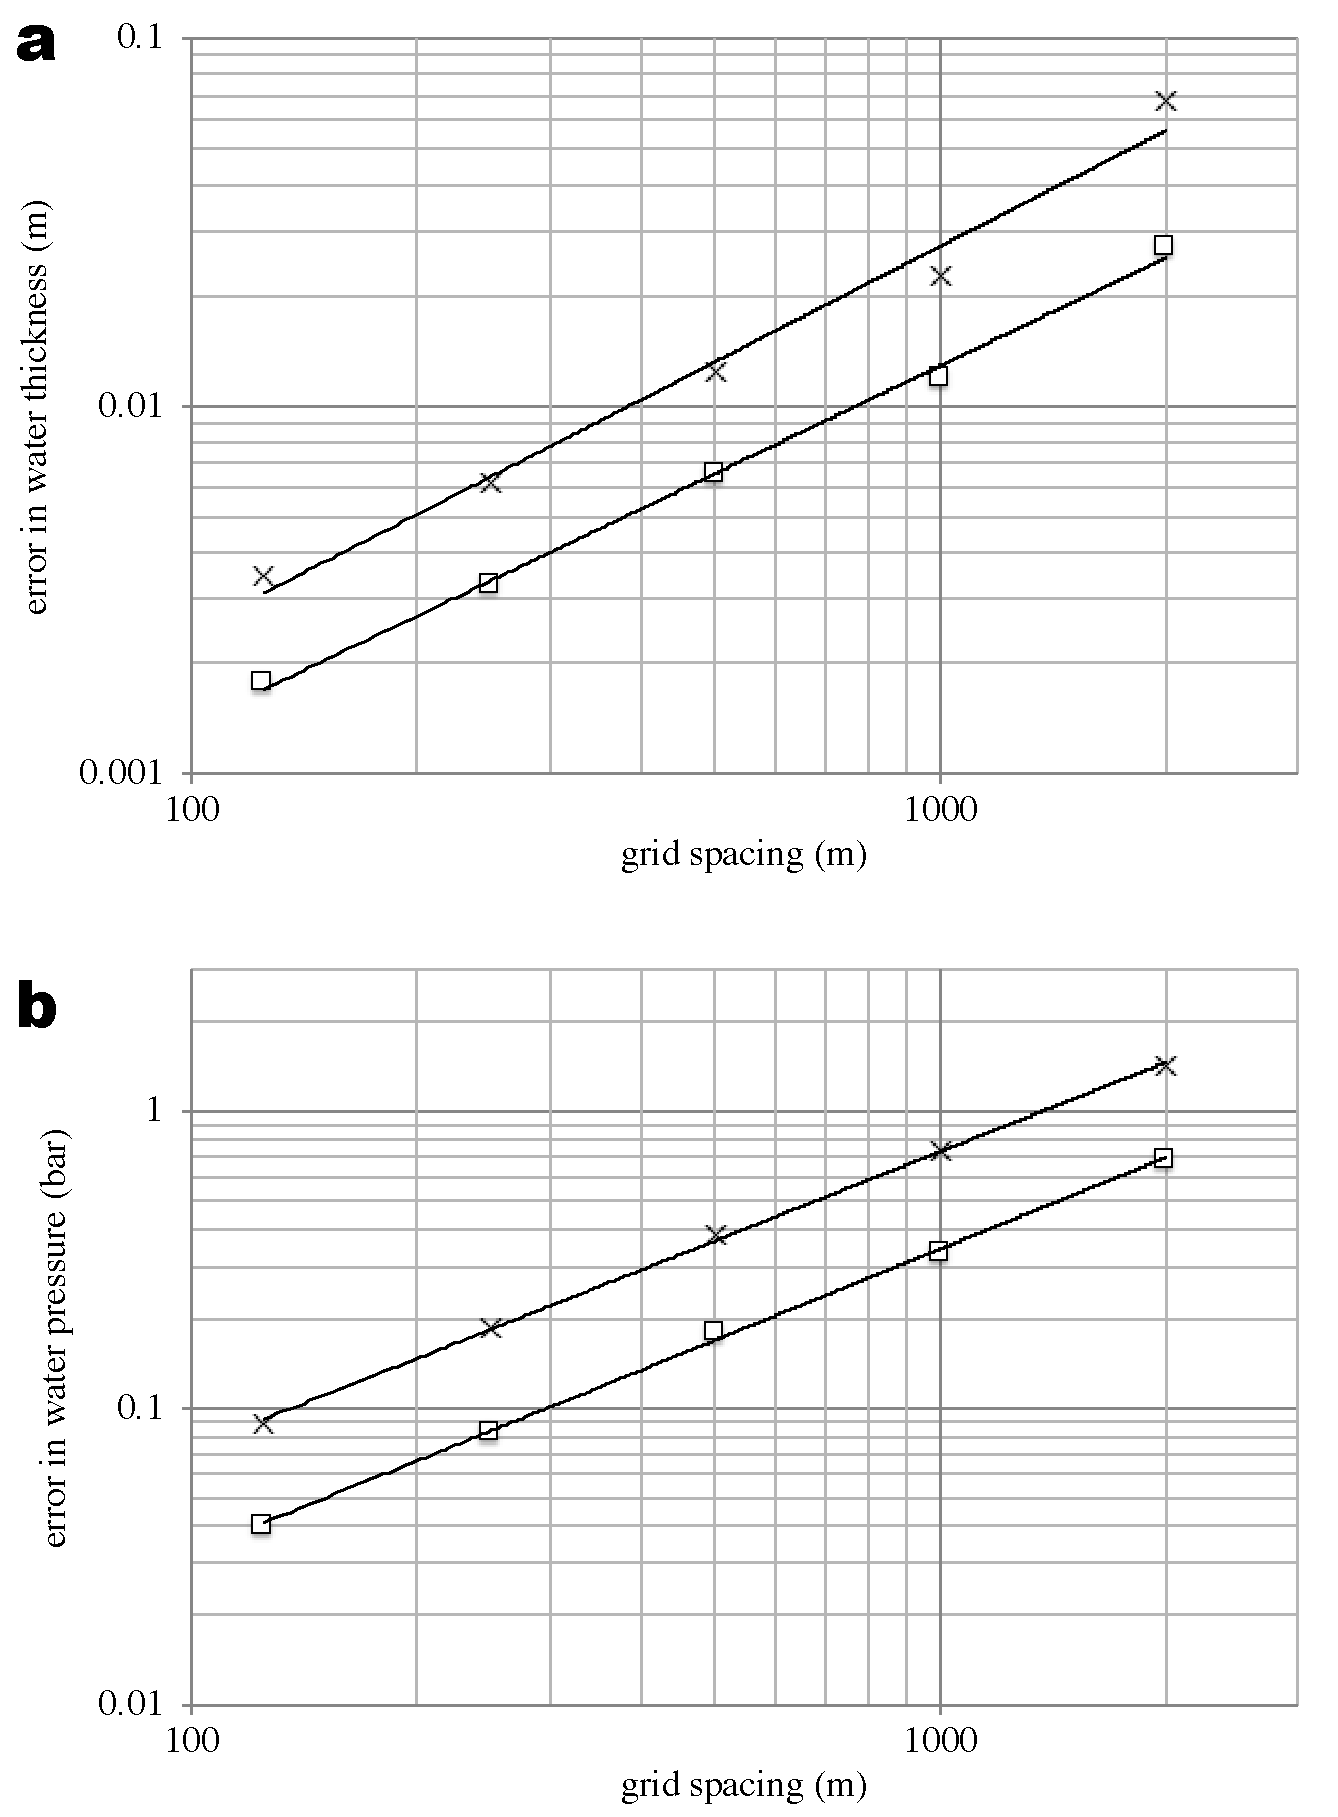
\includegraphics[width=8.0cm]{landice/figures/hydro_convergence_plots_clean.pdf}
\caption{
Error in subglacial hydrology model for radial test case with near-exact solution
described by \citet{Bueler2015} for different grid resolutions.
a) Error in water thickness.  $\times$ symbols indicate maximum error, and squares indicate mean error.
Average error in water thickness decays as $O(\Delta x^{0.97})$.
b) Error in water pressure, with same symbols.
Average error in water pressure  decays as $O(\Delta x^{1.02})$.
}
\label{fig:sgh:radialsolnfig}
\end{figure}

To check the model implementation of channels, we use comparisons to other, more mature drainage models
through the Subglacial Hydrology Model Intercomparison Project (SHMIP)\footnote{https://shmip.bitbucket.io/}.
Steady state solutions of the drainage system effective pressure, water fluxes, and channel development
for an idealized ice sheet with varying magnitudes of meltwater input (SHMIP experiment suites A and B)
compared between MALI and other models of similar complexity (GlaDS, Elmer) are very similar.

To demonstrate a real-world application of the subglacial hydrology model,
we perform a standalone subglacial hydrology simulation of the entire Antarctica Ice Sheet on a uniform 20 km resolution mesh (Figure \ref{fig:sgh:aisflux}).
We force this simulation with basal sliding and basal melt rate after optimizing the first-order velocity solver optimized to surface velocity observations (Figure \ref{fig:sgh:aisflux}a).
We then run the subglacial hydrology model to steady state with only distributed drainage active and using standard parameter values.
Results show a subglacial hydrologic state that is reasonable.
For example, the subglacial water flux shows similar spatial patterns to the basal sliding speed (Figure \ref{fig:sgh:aisflux}),
suggesting a basal friction law based on the subglacial hydrologic state could be configured to 
yield realistic ice velocity.
Calibrating parameters for the subglacial hydrology model and a basal friction law
and performing coupled subglacial-hydrology/ice-dynamics simulations are beyond the scope of this paper;
we merely mean to demonstrate plausible behavior from the subglacial hydrology model for a realistic ice-sheet-scale problem.

\begin{figure}[t]
\centering
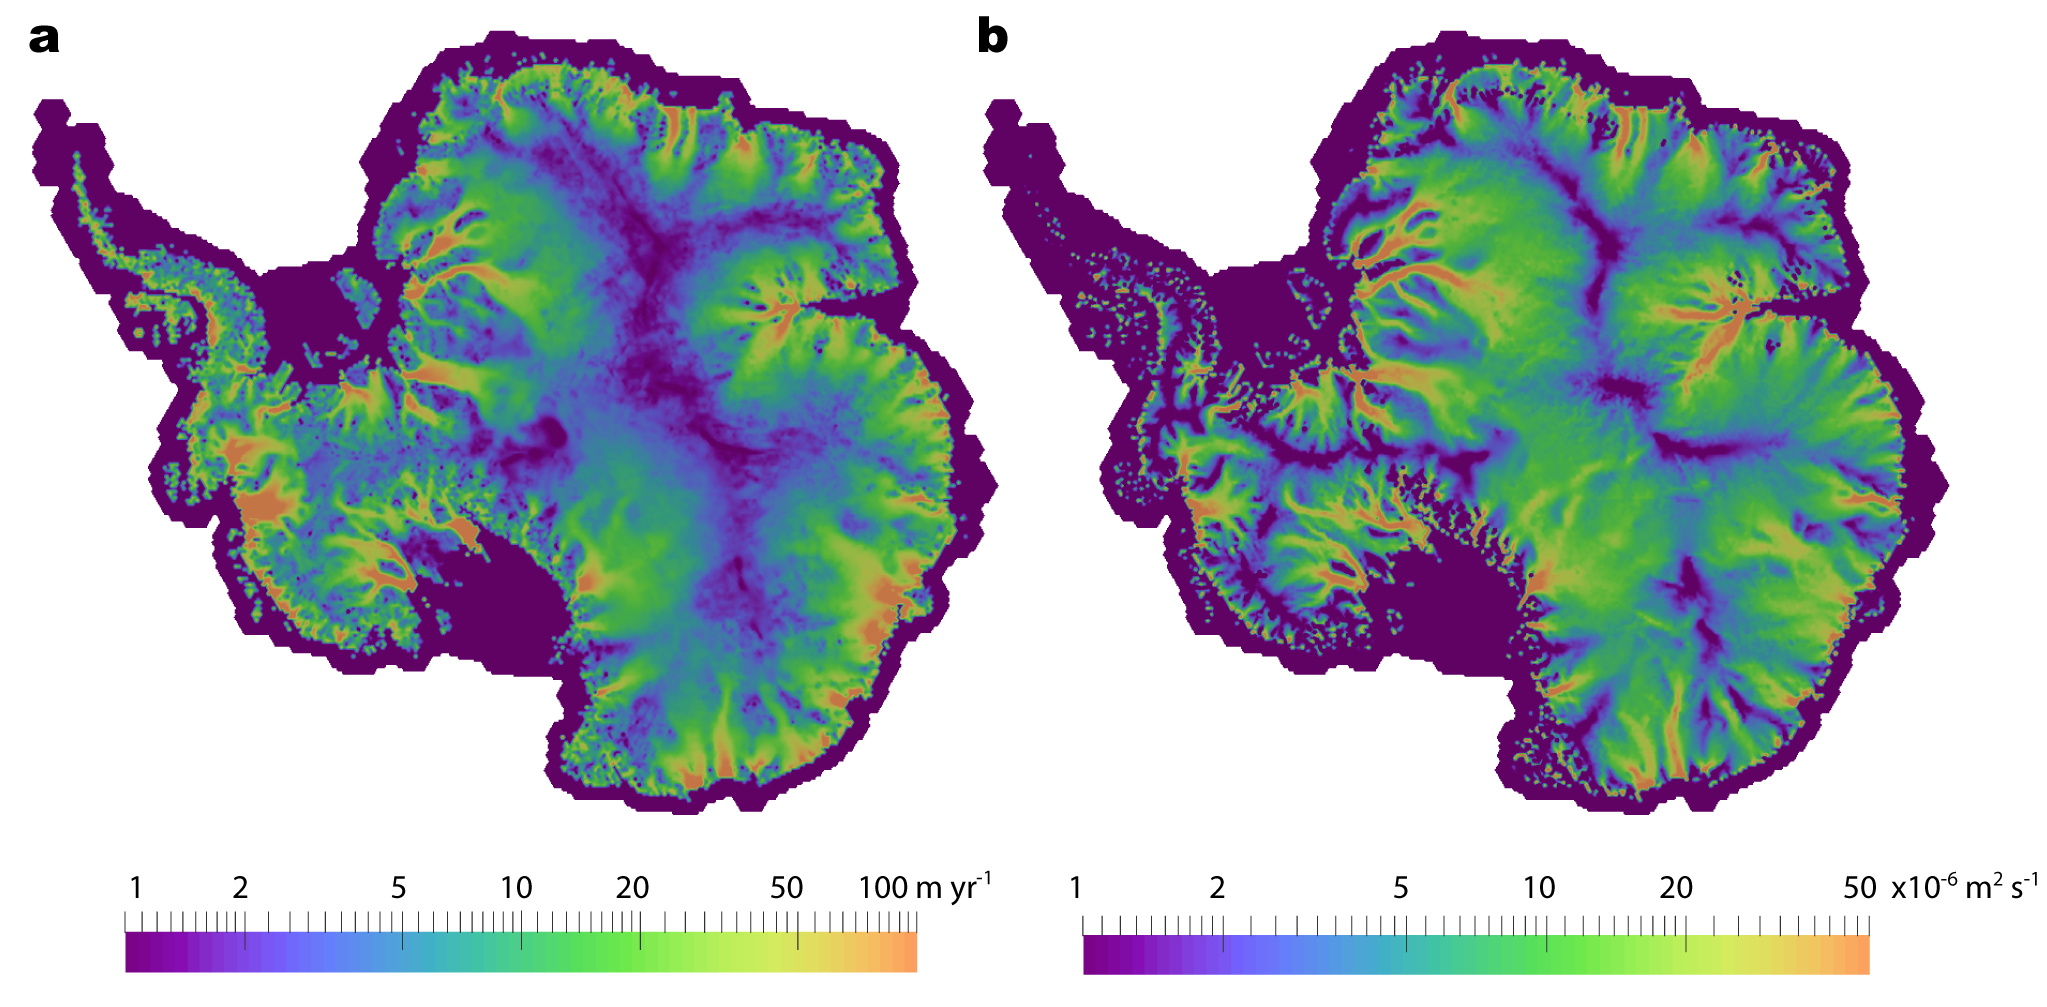
\includegraphics[width=15.3cm]{landice/figures/speed_vs_hydroflux_clean.png}
\caption{Subglacial hydrology model results for 20 km resolution Antarctic Ice Sheet. 
a) Basal ice speed calculated by the first-order velocity solver optimized to surface velocity observations.  This field and the calculated basal melt are the forcings applied to the standalone subglacial hydrology model.
b) Water flux  in the distributed system calculated by the subglacial hydrology model at steady state.
}
\label{fig:sgh:aisflux}
\end{figure}


% ========================
\section{Iceberg Calving}
% ========================
\label{sec:calving}
MALI includes a few simple methods for removing ice from calving fronts during each model time step:
\begin{enumerate}
\item All floating ice is removed.
\item All floating ice in cells with an ocean bathymetry deeper than a specified threshold is removed.
\item All floating ice thinner than a specified threshold is removed.
\item The calving front is maintained at its initial location by adding or removing ice after thickness evolution is complete. This option does \textit{not} conserve mass or energy but provides a simple way to maintain a realistic ice shelf extent (e.g., for model spinup).
\item ``Eigencalving'' scheme \citep{Levermann2012}.  Calving front retreat rate, $C_v$, is proportional to the product of the principal strain rates ($\dot{\epsilon_1}, \dot{\epsilon_2}$) if they both are extensional:
\begin{equation}
  C_v = K_2 \dot{\epsilon_1} \dot{\epsilon_2} \text{  for  } \dot{\epsilon_1} > 0 \text{  and  }   \dot{\epsilon_2} > 0.
\label{eigencalving}
\end{equation}
The eigencalving scheme can optionally also remove floating ice at the calving front with thickness below a specified thickness threshold \citep{Feldmann2015}.
In practice we find this is necessary to prevent formation of tortuous ice tongues and continuous, gradual extension of some ice shelves along the coast.
\end{enumerate}
Ice that is eligible for calving can be removed immediately or fractionally each time step
based on a calving timescale. 
To allow ice shelves to advance as well as retreat, we implement a simple parameterization for sub-grid motion of the calving front by forcing floating cells adjacent to open ocean to remain dynamically inactive until ice thickness there reaches 95\% of the minimum thickness of all floating neighbors.
This is an \textit{ad hoc} alternative to methods tracking the calving front position at sub-grid scales \citep{Albrecht2011,Bondzio2016}.
